\documentclass[a4paper,twoside]{article}

\usepackage{epsfig}
\usepackage{subcaption}
\usepackage{calc}
\usepackage{amssymb}
\usepackage{amstext}
\usepackage{amsmath}
\usepackage{amsthm}
\usepackage{multicol}
\usepackage{pslatex}
\usepackage{algorithm2e}
\usepackage[bottom]{footmisc}
% Please add other packages that you may need BEFORE the SCITEPRESS.sty package.
\usepackage{natbib}
\usepackage{multirow}
\usepackage{SCITEPRESS}
\usepackage{arydshln}
\widowpenalty=10000
\clubpenalty=10000

\begin{document}

\title{
  Analyzing Student Use of Spacing and Interleaving Strategies in Interactions
  with GenAI-Powered Chatbots in Programming Courses
}

\author{\authorname{Rodrigo Prestes Machado\sup{1}\orcidAuthor{0000-0003-0428-6387},
Carlos Alario-Hoyos\sup{2}\orcidAuthor{0000-0002-3082-0814},
Patricia Callejo\sup{2}\orcidAuthor{0000-0001-6124-6213},
Iria Estévez-Ayres\sup{2}\orcidAuthor{0000-0002-1047-5398},
Carlos Delgado Kloos\sup{2}\orcidAuthor{0000-0003-4093-3705}}
\affiliation{\sup{1}Department of Informatics, Instituto Federal de Educação,
Ciência e Tecnologia, Porto Alegre, Brazil}
\affiliation{\sup{2}Department of Telematics Engineering, Universidad Carlos III
de Madrid, Leganés (Madrid), Spain}
\email{\ rodrigo.prestes@poa.ifrs.edu.br, \{calario, pcallejo, ayres, cdk\}@it.uc3m.es}
}

\keywords{
  Programming, Generative Artificial Intelligence, Chatbots, Spacing,
  Interleaving and Metacognition
}

\abstract{
The aim of this study is to analyze the interactions of programming students
with a chatbot powered by OpenAI's GPT-3.5, enhanced with the Retrieval
Augmented Generation (RAG) technique, within the context of a Java programming
course. The study investigates how students use the chatbot while employing
two metacognitive strategies: interleaving and spacing. The methodology involved
classifying and categorizing the students' interaction prompts with the chatbot
into eight distinct categories. The findings reveal that, while most
interactions focus on active learning strategies, students demonstrate limited
conscious application of metacognitive strategies. The study highlights the need
for more comprehensive guidance on the strategic use of AI tools to enhance
learning outcomes.
}

\twocolumn\maketitle\normalsize\setcounter{footnote}{0}

\section{\uppercase{Introduction}}
\label{sec:introduction}

Recent advances in Generative Artificial Intelligence (GenAI) have created
new opportunities in both professional programming \citep{Peng23}
\citep{Pandey24} and education \citep{Puryear22}. In programming courses,
students can employ GenAI tools to improve their understanding, receive
personalized feedback, and access detailed explanations. For example, GitHub
Copilot, a tool that is integrated into development environments, assists in
providing real-time suggestions and accelerating code writing, which could help
streamline the learning process \citep{Denny23}. Educational chatbots, on the
other hand, try to guide students through coding challenges, answer questions,
and try to foster a deeper understanding of programming concepts
\citep{Labadze23}.

The study conducted by \cite{chan23} revealed that both undergraduate and
postgraduate students have positive attitudes towards the use of GenAI.
A systematic review organized by \cite{Lo24} demonstrated that students can
effectively learn from ChatGPT, resulting in improved comprehension and academic
achievement \citep{Callejo24}. Furthermore, it was observed that ChatGPT may
allow students to regulate their learning pace \citep{Baha24} and can
potentially support self-regulated learning, particularly for students with
prior technical and disciplinary knowledge \citep{Xia23}.

However, researchers have also expressed concerns about the impact of these
tools on students. The systematic review by \cite{Murillo23} indicated that the
use of ChatGPT could lead to overreliance on the tool. \cite{chan23} noted that
overdependence on ChatGPT could lead to a decrease in critical thinking, as
students can make decisions based solely on the information provided by the
tool. As a potential consequence, \cite{Bastani24} observed in a study that when
programming students lost access to ChatGPT, those who had previously relied
on it saw their performance drop by 17\%. In contrast, students who had never
used the tool were unaffected and outperformed their peers.

The confidence of students in these tools is well founded, as shown by
\cite{Puryear22}, who found that GitHub Copilot can generate solutions for
student assignments with precision rates ranging from 68\% to 95\%. However,
\cite{Boudouaia24} observed that using ChatGPT without a structured learning
approach did not provide significant improvement over traditional self-directed
learning methods in programming. This raises concerns that students may become
overly dependent on generative AI tools, potentially hindering their learning
progress and missing opportunities to develop a deeper understanding of
fundamental concepts.

Regardless of teachers' preferences or beliefs, preliminary surveys conducted
by \cite{Dickey24} indicate that more than 54.5\% of students are already using
GenAI for homework, likely due to their perception of this technology as
advantageous and intuitive \citep{Boudouaia24}. All of these studies highlight
the need to increase the understanding of how students interact with these tools
and how they can be used to improve learning, as emphasized by \cite{Lo24}.

In response to the growing need for deeper insight into the use of GenAI tools
in educational settings, this study aims to help address this gap by analyzing
the interactions between students in a Java programming course and an
educational chatbot powered by OpenAI gpt-3.5, enhanced with the
Retrieval-Augmented Generation (RAG) technique. Specifically, it focuses on
examining these interactions within the context of two metacognitive strategies:
spacing \citep{Carvalho20} and interleaving \citep{Rivers21}. To achieve this
objective, we formulate three research questions:

\begin{itemize}
  \item RQ1 - What distribution patterns emerged in the classified student
  interaction prompts with the educational chatbot?
  \item RQ2 - Was there spacing between student prompts? Which category led to
  the most rapid and consistent interactions with the chatbot?
  \item RQ3 - Do students' interactions with the chatbot alternate between study
  topics to suggest interleaving?
\end{itemize}

This paper is organized as follows. Section 2 presents the theoretical
framework, Section 3 describes the material and methods used in the study,
Section 4 presents the results and discussion, and Section 5 concludes the
paper and outlines future work.

\section{\uppercase{Theoretical Framework}}

This section outlines the theoretical framework that is the basis of the study.
We begin by introducing the concept of metacognition, along with the spacing and
interweaving strategies applied in this research. Next, we present related works
organized into two subsections: research involving GenAI and studies focusing
on metacognition.

\subsection{Metacognition}

Given that GenAI often produces highly accurate and automatic responses
\citep{Puryear22}, it is essential that students use these tools within an
active learning process to enhance their learning outcomes. This active
learning process can be further understood through the lens of metacognition,
which focuses on awareness of one's mental processes. \cite{flavell79}
proposed a model of metacognitive monitoring that includes four interrelated
phenomena: Metacognitive Knowledge, Metacognitive Experience, Metacognitive
Goals, and Metacognitive Actions. These processes do not occur in isolation, but
they influence each other, altering cognitive progress over time.

Metacognitive knowledge includes beliefs about variables that affect the
outcomes of cognitive activities. It is divided into three types: beliefs about
personal abilities, perceived difficulty in the task, and previously used
strategies. Metacognitive Experience refers to the feelings that arise before,
during, and after cognitive activity, such as frustration, confusion,
satisfaction, and others. Metacognitive Goals are the key to regulating thought
as they relate to the goals the individual seeks to achieve, directly
influencing the actions taken. For example, if a student’s goal is to complete
a task quickly, they may adopt a more passive approach to learning. Lastly,
Metacognitive Actions involve the planning, monitoring, and evaluation of
strategies used to achieve the goals. In terms of planning, students can
determine how to approach a task, such as spacing their study sessions
\citep{Ouhao18, Carvalho20}, interleaving topics \citep{Rivers21}, utilizing
retrieval practice \citep{larsen18}, and other possible strategies.

Spacing and interleaving are two metacognitive strategies that have been shown
to enhance learning outcomes and support the research questions of this study.
Spacing refers to the practice of distributing study sessions over time, which
has been shown to improve long-term retention and understanding of the material
\citep{Carvalho20}. Interleaving involves mixing different topics or problems
within a single learning session, which has been shown to also enhance long-term
learning and the application of student's knowledge in other contexts and
situations \citep{Rivers21}.

\subsection{GenAI Related Works}

\cite{Margulieux24} conducted a study on how undergraduate students in
introductory programming courses used generative AI to solve programming
problems in a naturalistic setting. The research focused on examining the
relationship between AI usage and students’ self-regulation strategies,
self-efficacy, and fear of failure in programming. Furthermore, the study
explored how these variables interacted with the characteristics of the learners,
the perceived usefulness of AI, and academic performance. The findings revealed
that students with higher self-efficacy, lower fear of failure, or higher prior
grades tended to use AI less frequently or later in the problem-solving process
and perceived it as less useful compared to their peers. However, no significant
relationship was found between students’ self-regulation strategies and their
use of AI.

\cite{Boudouaia24} investigated the impact of ChatGPT-facilitated programming on
college students’ programming behaviors, performance, and perceptions. The
problem addressed was whether the use of ChatGPT in programming education could
influence how students interacted with programming tasks, their learning
outcomes, and their attitudes towards technology. The study employed a
quasi-experimental design involving 82 college students divided into two groups:
one using ChatGPT-assisted Programming (CAP) and the other using traditional
self-directed Programming (SDP). The method combined mixed data collection
techniques, including behavioral logs, programming performance evaluations, and
interviews. The results showed that students using the CAP mode exhibited more
frequent behaviors such as debugging and reading feedback. Although CAP students
had a higher average score in programming performance, there was no
statistically significant difference compared to the SDP group. However,
students’ perceptions of ChatGPT improved significantly after the intervention,
with increased perceived usefulness, ease of use, and intention to continue
using the tool in the future.

\cite{Bastani24} investigated the impact of GenAI, specifically GPT-4, on human
learning, with a focus on mathematics education in a high school. The problem
addressed was how the use of generative AI could affect the acquisition of new
skills, which is crucial for long-term productivity. The method involved a
controlled experiment with approximately one thousand students, who were exposed
to two GPT-4-based tutors: a simple tutor (GPT Base) and another with safeguards
designed to promote learning (GPT Tutor). The results showed that while access
to GPT-4 improved performance on practice exercises (48\% with GPT Base and
127\% with GPT Tutor), the removal of access to GPT Base led to a 17\% decrease
in student performance on exams. This suggests that unrestricted use of
\textit{GPT Base} could hinder learning. However, the GPT Tutor was able to
mitigate this negative effect.

\begin{table*}[htbp]
  \caption{Categories - adapted from \cite{Ghimire24}}
  \begin{center}
    \renewcommand{\arraystretch}{1.6} % Increase the spacing between rows
    \begin{tabular}{p{4cm} p{12cm}} % Remove vertical bars
      \hline
      \textbf{Category} & \textbf{Description} \\
      \hline
      Debugging Help (DH) & Prompts that seek help to identify, fix errors, or understand the provided code snippet. \\
      Conceptual Question (CQ) & Prompts that are more about understanding concepts than specific code. \\
      Student Correction (SC) & Prompts where the student corrects the chatbot. \\
      Code Snippet  (CS) & Prompts that ask for a specific part of the code, like a function or a segment. \\
      Complete Solution (CSO) & Prompts that request an entire solution or a complete code snippet. \\
      Multiple Question (MQ) & Prompts where the user wants to solve a multiple choice exercise (Quiz). \\
      Language Change (LC) & Prompts that request a change of idiom. \\
      Uncategorized (U) & Prompts that do not fit into any of the above categories. \\
      \hline
    \end{tabular}
    \label{tab:categories}
  \end{center}
\end{table*}

\subsection{Metacognition Related Works}

Learning based on metacognitive strategies has been shown to be effective in
enhancing students’ performance and skills. \cite{Zheng19} investigated the
effects of metacognitive scaffolds on group behavior, performance, and cognitive
load in computer-supported collaborative environments. The results showed
positive impacts on metacognitive behavior and group performance without
increasing the cognitive load. \cite{LiWei23} proposed a metacognition-based
collaborative approach to enhance performance in collaborative programming. The
findings indicated that this approach influenced computational thinking,
critical thinking, and metacognitive awareness. Similarly, \cite{Wang23}
explored how metacognitive instruction affects computational thinking, critical
thinking, and metacognitive skills in collaborative programming, observing
improvements in problem-solving and collaboration. \cite{Khusnul24} investigates
the efficacy of a meta-learning approach in improving metacognitive and creative
skills. This study confirms the effectiveness of metacognition strategies and
elucidates the relationship between meta-learning and metacognition. This
research suggests that meta-learning can improve metacognitive abilities,
providing valuable insights into educational technology and course design in
higher education settings.

\cite{Sidra24} addressed the growing importance of metacognitive skills in an
AI-enabled workforce. The problem discussed was how AI systems, especially in
collaborative tools based on Large Language Models (LLMs), impacted human
decision-making and the challenges they posed due to the lack of human-like
metacognition in AI. The method used identified four main characteristics that
differentiated human-AI interaction from human-human collaboration and proposed,
based on the dual-process theory of human thought, that metacognitive thinking
was crucial for the effective use of AI. The results indicated that human
workers needed to develop and apply metacognitive skills, such as planning,
monitoring, and evaluating their thought processes, to mitigate cognitive biases
and improve decision-making when working with AI. The study concluded by
recommending improvements in AI design and training to improve workers'
metacognitive abilities, ensuring more effective collaboration with AI systems.

\section{\uppercase{Material and Method}}

This section outlines the tools and procedures used in this study. CharlieBot
served as the GenAI tool for educational purposes, and the method was structured
into three distinct phases, each designed to systematically assess its
interaction with students.

\subsection{CharlieBot}

CharlieBot is an educational chatbot built on ChatGPT 3.5 and enhanced with
Retrieval-Augmented Generation (RAG) technique to improve the precision of
responses provided to students \citep{Sun24}. The RAG approach was developed
using materials from a MOOC, including text, exercises, video transcripts, and
other resources.

\subsection{Method}

The study comprised three phases: data collection, categorization, and analysis.
During the data collection phase, students enrolled in a second-semester Java
course at a public university in Spain were introduced to CharlieBot and given
the freedom to use it without following any prescribed educational methodology.
All data were collected anonymously to ensure that interactions could not be
traced back to individual students or linked to their academic performance.

In the categorization phase, the students' messages were manually classified
into eight distinct categories for analysis, representing different types of
prompt that students use when interacting with the chatbot. Initially,
\cite{Ghimire24} proposed four categories: Debugging Help (DH), Conceptual
Question (CQ), Code Snippet (CS), and Complete Solution (CSO). However, the data
collected indicated the need for additional categories, leading to the inclusion
of four more: Multiple Question (MQ), Student Corrections (SC), Language Change
(LC), and Uncategorized (U). In this study, students were free to use the
chatbot as they wanted, which contributed to the emergence of these additional
categories. Table \ref{tab:categories} presents these categories along with
their respective descriptions. To facilitate the analysis, the prompt topics
were also categorized according to the course subjects, which are: (1) Java, (2)
Object Orientation, (3) Testing, (4) Recursion, (5) Data Structures, and (6)
Sorting and Searching Algorithms.

The analysis phase involved the use of Python scripts to extract information
from previously classified data. The data sets and code used in this process are
available at: https://github.com/rodrigoprestesmachado/uc3m.

\section{\uppercase{Results and Discussion}}

A total of 625 student messages were categorized in 81 conversations, with
an average of 7.72 messages per conversation. This data offers insights into how
users engage with CharlieBot and the types of prompts they submit. The results
of the analysis are presented in this section, addressing the research questions
outlined in the introduction. Figure \ref{fig:graph1} shows the distribution of
the messages in the categories. The following sections present the results and
discussions of each research question.

\subsection{Categorization of messages}

About the first research question: \textit{RQ1 - What distribution patterns
emerged in the classified student interaction prompts with the educational
chatbot?}

According to Figure \ref{fig:graph1} messages classified as
Conceptual Question account for 35.8\% of the total. Sequences of Conceptual
Questions often start from a practical perspective of a given code, as
illustrated in conversation 4 of Figure \ref{fig:graph2}, which presents
examples of students' interactions with the chatbot. In other cases, the
conversation consists entirely of messages classified as Conceptual Question,
such as in conversation 15 of Figure \ref{fig:graph2}.

\begin{figure}[h!]
  \centering
  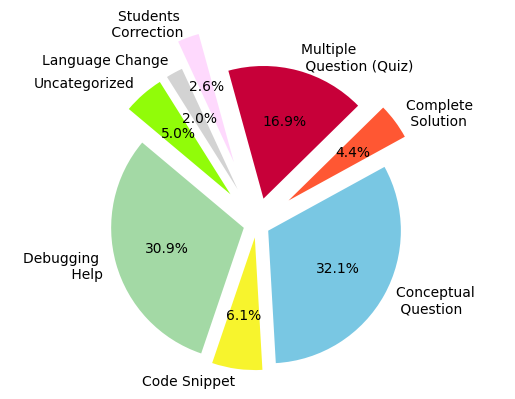
\includegraphics[scale=0.62]{img/figure1.png}
  \caption{Categorization of messages.}
  \label{fig:graph1}
\end{figure}

\begin{figure*}[htbp]
  \centering
  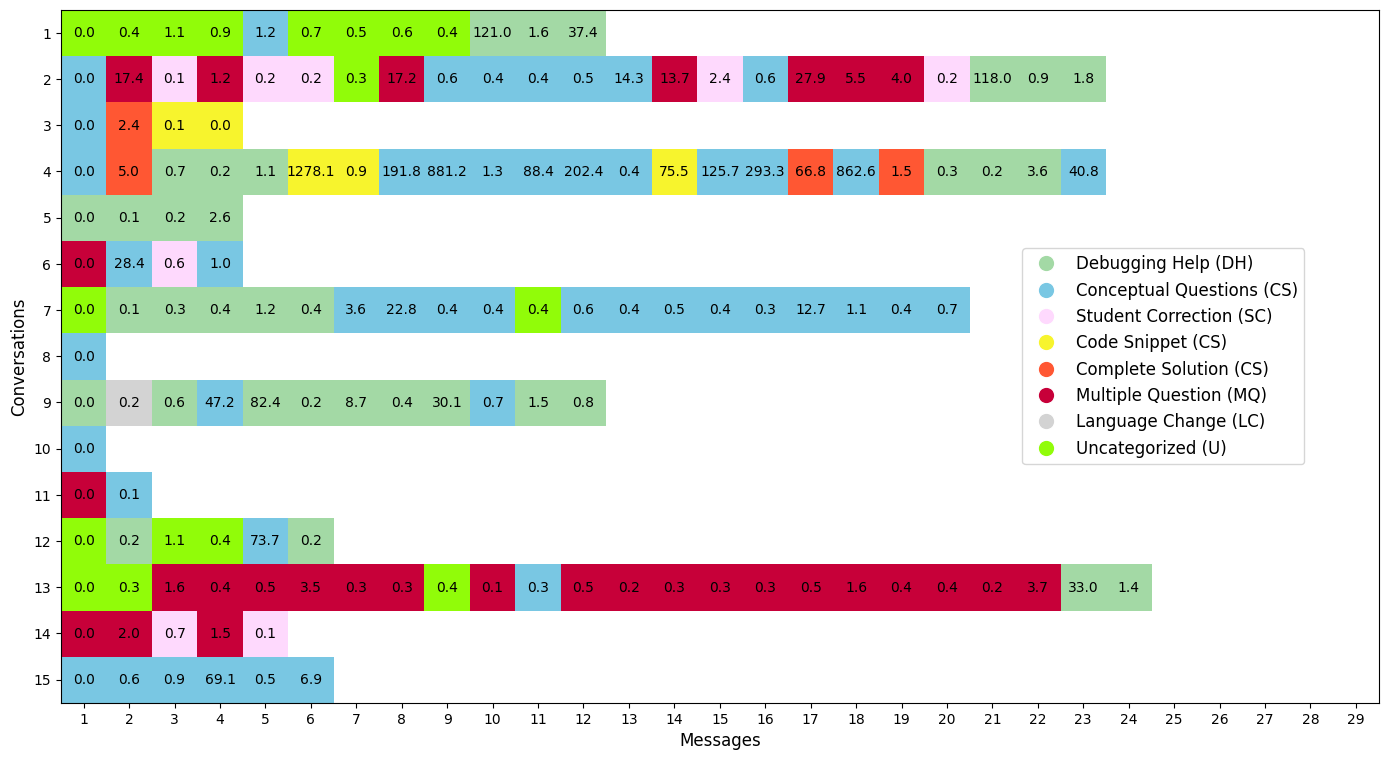
\includegraphics[scale=0.45]{img/figure2.png}
  \caption{Examples of conversations.}
  \label{fig:graph2}
\end{figure*}

As shown in Figure \ref{fig:graph1}, approximately 29.9\% of the messages were
classified as Debugging Help. Debugging help messages are likely to provide
students with a practical approach to understanding code, identifying errors,
and building skills to enhance their debugging abilities for future tasks.

Most of the messages are located in the categories Conceptual Question and
Debugging Help corroborate the findings of \cite{Ghimire24} which showed that
the questions are also localized in the same categories.

Multiple Question exercise resolutions represented 14.9\% of the responses.
These prompts typically involved students submitting one or more exercises to
CharlieBot and requesting solutions. The conversation 13 in Figure
\ref{fig:graph2} illustrates a sequence of multiple choice questions.

Requests for the chatbot to generate a Code Snippet or Complete Solution accounted
for 8.2\% of student messages. These prompts reflected a desire for more
direct answers; however, it was observed that, after receiving these solutions,
many students transitioned to a more active approach in seeking to understand
the code or the underlying concepts. Thus, it can be inferred that the prompts
within the Code Snippet or Complete Solution category were often used as a
starting point for a more in-depth study.

Student corrections to chatbot responses represented 4.2\% of the interactions.
In most cases, these corrections occurred when the student already had the
correct answer to an exercise and identified an error in the chatbot response,
as illustrated in conversation 2 in Figure \ref{fig:graph2}. These corrections
highlight that, although the chatbot provides quick feedback, it is not always
accurate.

Figure \ref{fig:graph1} also indicates that approximately 5.8\% of the prompts
written by the students were classified as Uncategorized. These messages include
expressions of gratitude toward the chatbot, such as a simple '\textit{thanks}',
contextual statements like '\textit{I'm reviewing object orientation}', as well
as requests for additional exercises and summaries. Depending on the type of
investigation, there is opportunity for these messages to be further subdivided
into new categories.

Finally, 1.3\% of the messages were classified as Language Change. These prompts
were typically requests for the chatbot to switch languages, as seen in
conversation 9 in Figure \ref{fig:graph2}.

\subsection{Spacing}

About the first part of the second research question: \textit{RQ2 - Was there
spacing between student prompts?}

For the analysis of the spacing, we initially considered a minimum interval of
60 minutes as a reference to define the significant spacing \citep{Gadella24}.
Based on this, our results showed that, of the 81 conversations analyzed, only
27 (33.3\%) had at least one message with an interval greater than 60 minutes.
Figure 2 illustrates the elapsed time between messages (delta). For example,
in conversation 15, the first message was sent at time zero, while the second
message was sent by the student after a delta of 0.6 minutes. Additionally,
message 4 in conversation 15, as shown in Figure \ref{fig:graph2}, presents a
delta of 69.1 minutes, which, according to our reference, characterizes
significant spacing. Figure \ref{fig:graph3} also shows the number of spacings
in each conversation. Among conversations that exhibited spacing, the
average number of subsections per conversation was 2.2. Therefore, a
conversation with one instance of spacing is typically divided into two distinct
study subsections.

This data suggests that there is indeed little spacing between study sessions.
It is worth noting that, in order to create a new section in CharlieBot,
students must close the browser tab and start a new conversation, which results
in losing the previous chat history.

\subsubsection{Interaction Time per Category}

About the second part of the second research question: \textit{RQ2 - Which
category led to the most rapid and consistent interactions with the chatbot?}

When a student requests a code snippet (CS), it is generally predictable that
they will resume interaction with the chatbot within a short period of time, as
indicated by the mean (1.26) and standard deviation (1.74) of the Code Snippet
category in Table \ref{tab:averages}. This result is noteworthy because,
although some requests are simple and lead to quick responses, others may be
more complex and would require more time for reflection. However, the low
average response time and minimal variability may indicate that students adopt a
more passive learning posture when requesting the chatbot to generate small pieces
of code.

\begin{figure*}[htbp]
  \centering
  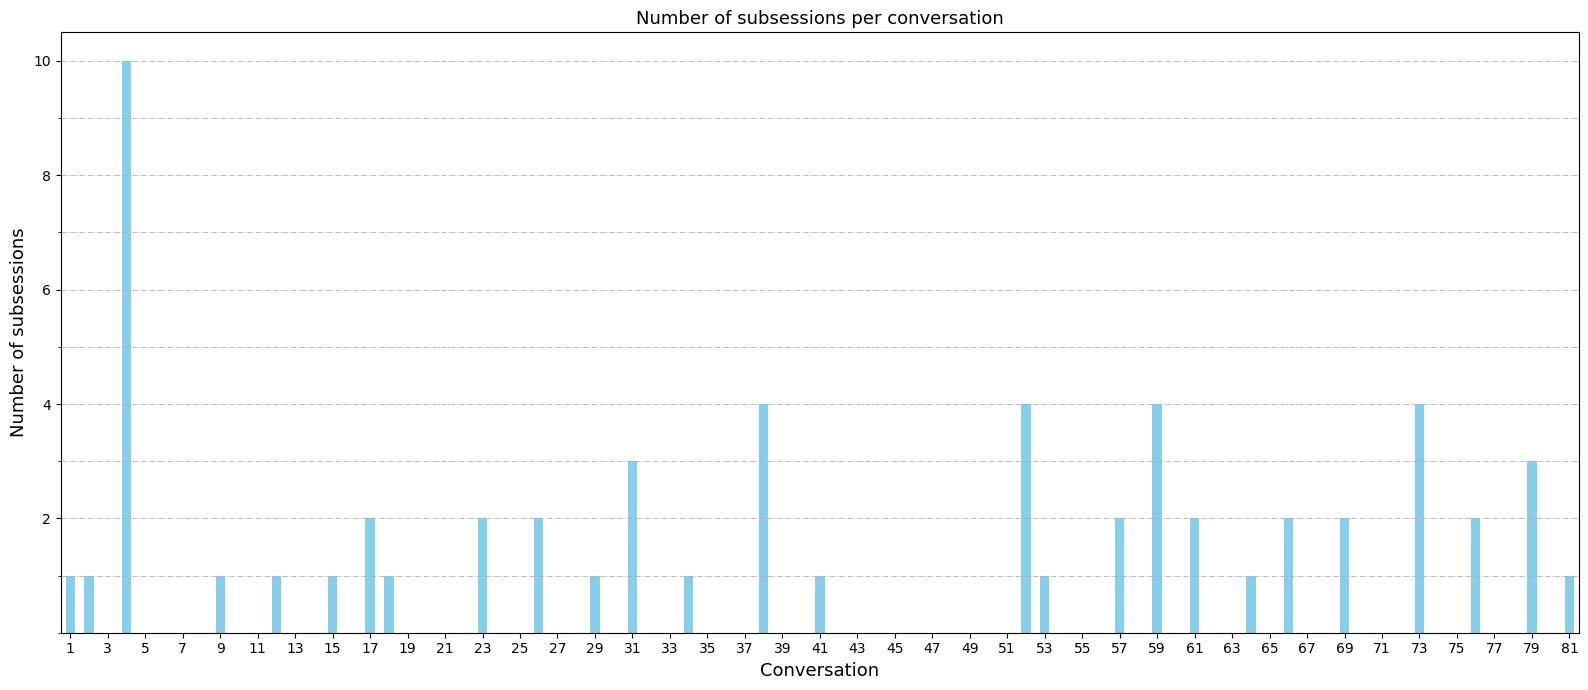
\includegraphics[scale=0.39]{img/figure3.png}
  \caption{Subsections per conversation. \textit{A zero value indicates
  no subsection and no spacing.}}
  \label{fig:graph3}
\end{figure*}

Despite some occasional variation (3.54), prompts classified as Uncategorized
exhibit a relatively low average time (1.65) for students to resume interaction
with the chatbot. This variation occurs, in part, because of situations where students
end the conversation with an uncategorized message, such as a simple
\textit{"thanks"}, but later choose to resume the interaction.

When a student requests the chatbot to change the language (LC) in a response, the
new interaction occurs quickly (1.89) with little variation in response time
(3.28), meaning that it is predictable that the student will continue interacting.

Although still below the overall average, students take a moderate amount of
time (2.65) to resume interaction with the chatbot after requesting the solution to
a multiple-choice question (MQ). The variation (6.10) suggests that some
responses may lead to a slower follow-up interaction, possibly indicating a
moment of deeper reflection on the part of the students. However, since both the
mean and standard deviation are below the overall average, this could indicate
a more passive behavior, as students obtain ready-made answers from the chatbot.

The average time for students to resume interaction in the correction category
(SC) is close to the overall average (3.17), although the high standard
deviation (7.33) indicates significant variation. In some cases, students are
already familiar with the answer and only seek a quick correction from the chatbot;
in others, they detect flaws in the chatbot's responses and need to carefully
examine the subsequent answer to identify potential errors, which suggests a
more active behavior.

After a question classified as Debugging Help (DH), there is both a
longer-than-average response time (4.84) and a high variation in the time taken
for a new interaction (10.13). This suggests that student prompts in this
category tend to be more time-consuming and unpredictable. A possible
explanation is that some DH issues are simple, such as '\textit{what does x++ do?}',
while others involve requests for analysis of more complex code, like
\textit{'explain this piece of code (accompanied by a complete method).'}

Conceptual questions (CQ) generally result in a high average time (5.41) for
students to reengage with the chatbot. Moreover, the high standard deviation
(10.54) indicates an unpredictable variation in response times. This
unpredictability may be attributed to the fact that, in some cases, the
complexity of the question and answer demands more reflection time from the
student, whereas in others, lesser complexity allows for a quicker interaction
with the chatbot.

Finally, a message classified as a Complete Solution request (SCO) exhibits the
longest average time (6.55) for students to resume interaction with the chatbot.
Additionally, the high standard deviation (10.14) highlights significant
unpredictability in response time. After requesting a complete solution,
students tend to take longer to return due to the complexity of the problems
involved, such as the implementation of sorting algorithms such as Heapsort. Table
\ref{tab:averages} presents the means and standard deviations for each
category.

However, some categories suggest quicker interactions with less reflection on
the part of students, such as 'Code Snippet' and 'Multiple Choice.' On the other
hand, other categories indicate that students may be in a more reflective
process, such as 'Debugging Help,' 'Conceptual Question,' and 'Complete
Solution.' This demonstrates that the level of student engagement varies
according to the nature of the requested interaction, reflecting different
approaches and depths in the learning process.

\begin{table*}[htbp]
  \caption{Average and Standard Deviation of Different Categories (in minutes)}
  \begin{center}
    \renewcommand{\arraystretch}{1.6} % Increase the spacing between rows
    \begin{tabular}{p{4cm} p{4cm} p{4cm}} % Remove vertical bars
      \hline
      \textbf{Category} & \textbf{Average} & \textbf{Standard Deviation} \\
      \hline
      Code Snippet & 1.26 & 1.74 \\
      Uncategorized & 1.65 & 3.54 \\
      Language Change & 1.89 & 3.28 \\
      Multiple Question & 2.65 & 6.10 \\
      Student Correction & 3.17 & 7.33 \\
      \hdashline
      \textit{Overall} & \textit{3.43} & \textit{6.60} \\
      \hdashline
      Debugging Help & 4.84 & 10.13 \\
      Conceptual Questions & 5.41 & 10.54 \\
      Complete Solution & 6.55 & 10.14 \\
      \hline
    \end{tabular}
    \label{tab:averages}
  \end{center}
\end{table*}

\subsection{Interleaving}

About the third research question: \textit{RQ3 - Do students' interactions with
the chatbot alternate between study topics to suggest interleaving?}

To analyze the interweaving of topics, sections were initially divided into
those that exhibited spacing and those that did not.

In conversations with the chatbot that did not include spacing (66.7\% of the total
conversations), approximately 19.2\% of the messages resulted in a change of
topic. Qualitative analysis of what led to this interweaving indicates that
part of it was due to students' requests for assistance in solving exercises
from different topics, suggesting a less active learning approach, as the time
interval for this type of interaction tends to be shorter than average.
Additionally, some instances of interweaving were observed after a prolonged
period of 20 to 50 minutes, still below the 60-minute threshold established as
the cutoff for considering spacing.

In interactions with the chatbot that included spacing (33.3\% of the total
conversations), approximately 31.4\% of the messages switched topics.
Qualitative analysis of these interactions reveals that a significant portion
of this interweaving was caused by spacing. In other words, some students use
the chatbot for quick consultations, asking a question and then returning hours
later with another question on a different subject.

Thus, the data revealed that the existing interweaving is limited and does not
suggest an effective study strategy, as it mainly arises from requests for
exercise resolution and from the natural spacing pattern of a consultation
interaction.

\section{Conclusion and Future Work}

The objective of this work was to analyze the interactions of Java programming
students with an educational chatbot developed using the RAG technique, employing
two metacognitive study strategies: spacing and interleaving.

The metacognition theory, along with the classification of student actions,
proved to be effective in understanding and revealing how students use the chatbot.
The results showed that most messages fall into the categories of Conceptual
Questions and Debugging Help, both known for promoting slower engagement and
potentially fostering more active learning. However, the results also indicated
that students' use of study strategies such as spacing and interleaving remains
limited, from which we can conclude that encouraging students to apply these
strategies more intentionally could enhance their learning while using GenAI.

It is important to consider how GenAI tools impact students in various
demographic groups, academic disciplines, cultural backgrounds, and levels of
previous experience \citep{catalan21} \citep{neo22}. Consequently, this study is
limited to a specific group of students and focuses on the use of a single GenAI
tool. As a result, the findings may not be generalizable to other populations or
tools.

To further explore this, a broader study is planned to examine, for instance,
the relationship between student profiles, use of metacognitive scaffolds, their
effective study strategies in using a GenAI, and learning outcomes.
In addition, to help educators analyze student behavior and provide
more targeted assistance, an AI model is being developed to automatically
classify student messages, offering valuable information on how these tools are used.

\bibliographystyle{apalike}
{\small
\bibliography{References}}

\end{document}
